\clearpage
\section{Closure tests and systematic uncertainties on transfer factors\label{sec:bkgd-syst}}

Limitations in simulating detector effects and event kinematics 
requires us to apply appropriate systematic uncertainties 
on the simulation-based translation factors. The following section 
describes how we obtain these uncertainties through the method of closure tests.

\subsection{Closure tests\label{sec:closure-tests-desc}}

At its core, the method compares an observed yield (\nobs) and a predicted
yield (\npre) in a sub-sample of a control region.  The predicted yield is constructed
by translating from a statistically independent data sample to the data sample of
interest by the use of the proper translation factor.  For example, in a given HT bin,
a prediction for the \njethigh, \nb=1, \mj sample can be made by translating from the
\njetlow, \nb=1, \mj in data via the translation factor: 
\begin{equation}
  \label{equ:tf-ratio-closure}
  \frac{N_{\rm MC}^{\rm \mj}(\scalht,\njethigh, \nb=1)}{N_{\rm MC}^{\rm \mj}(\scalht,\njetlow,\nb=1)} 
\end{equation}

The agreement between \nobs and \npre is expressed as $(\nobs - \npre)/\npre$.
Assuming only statistical uncertainties on \nobs and \npre, deviation of the 
ratio from zero defines our level of closure. A closure test set is defined
as ratios for each \scalht bin. Looking at the ratio as a function
of \scalht allows the measurement of statistical significant biases from zero and/or 
any dependence on \scalht.  If statistically significant biases
are observed, further studies are required to understand and correct
for these biases.

Eight sets of closure tests probe key ingredients of the simulation modeling 
of the SM backgrounds with genuine \met as a function of \scalht, as shown in
Fig.~\ref{fig:closure}. This is done for the two jet multiplicity bins
separately: (a) $2 \leq \njet \leq 3$ and (b) $\njet \geq 4$.

Under the assumption of closure for the full ensemble of tests,
systematic uncertainties on the transfer factors are derived for each
\njet category and \scalht regions. The treatment for
estimating the systematic uncertainties on the transfer factors is
described in Section~\ref{sec:syst-from-closure}.

\begin{figure}[h!]
  \begin{center}
    \subfigure[$2 \leq \njet \leq 3$]{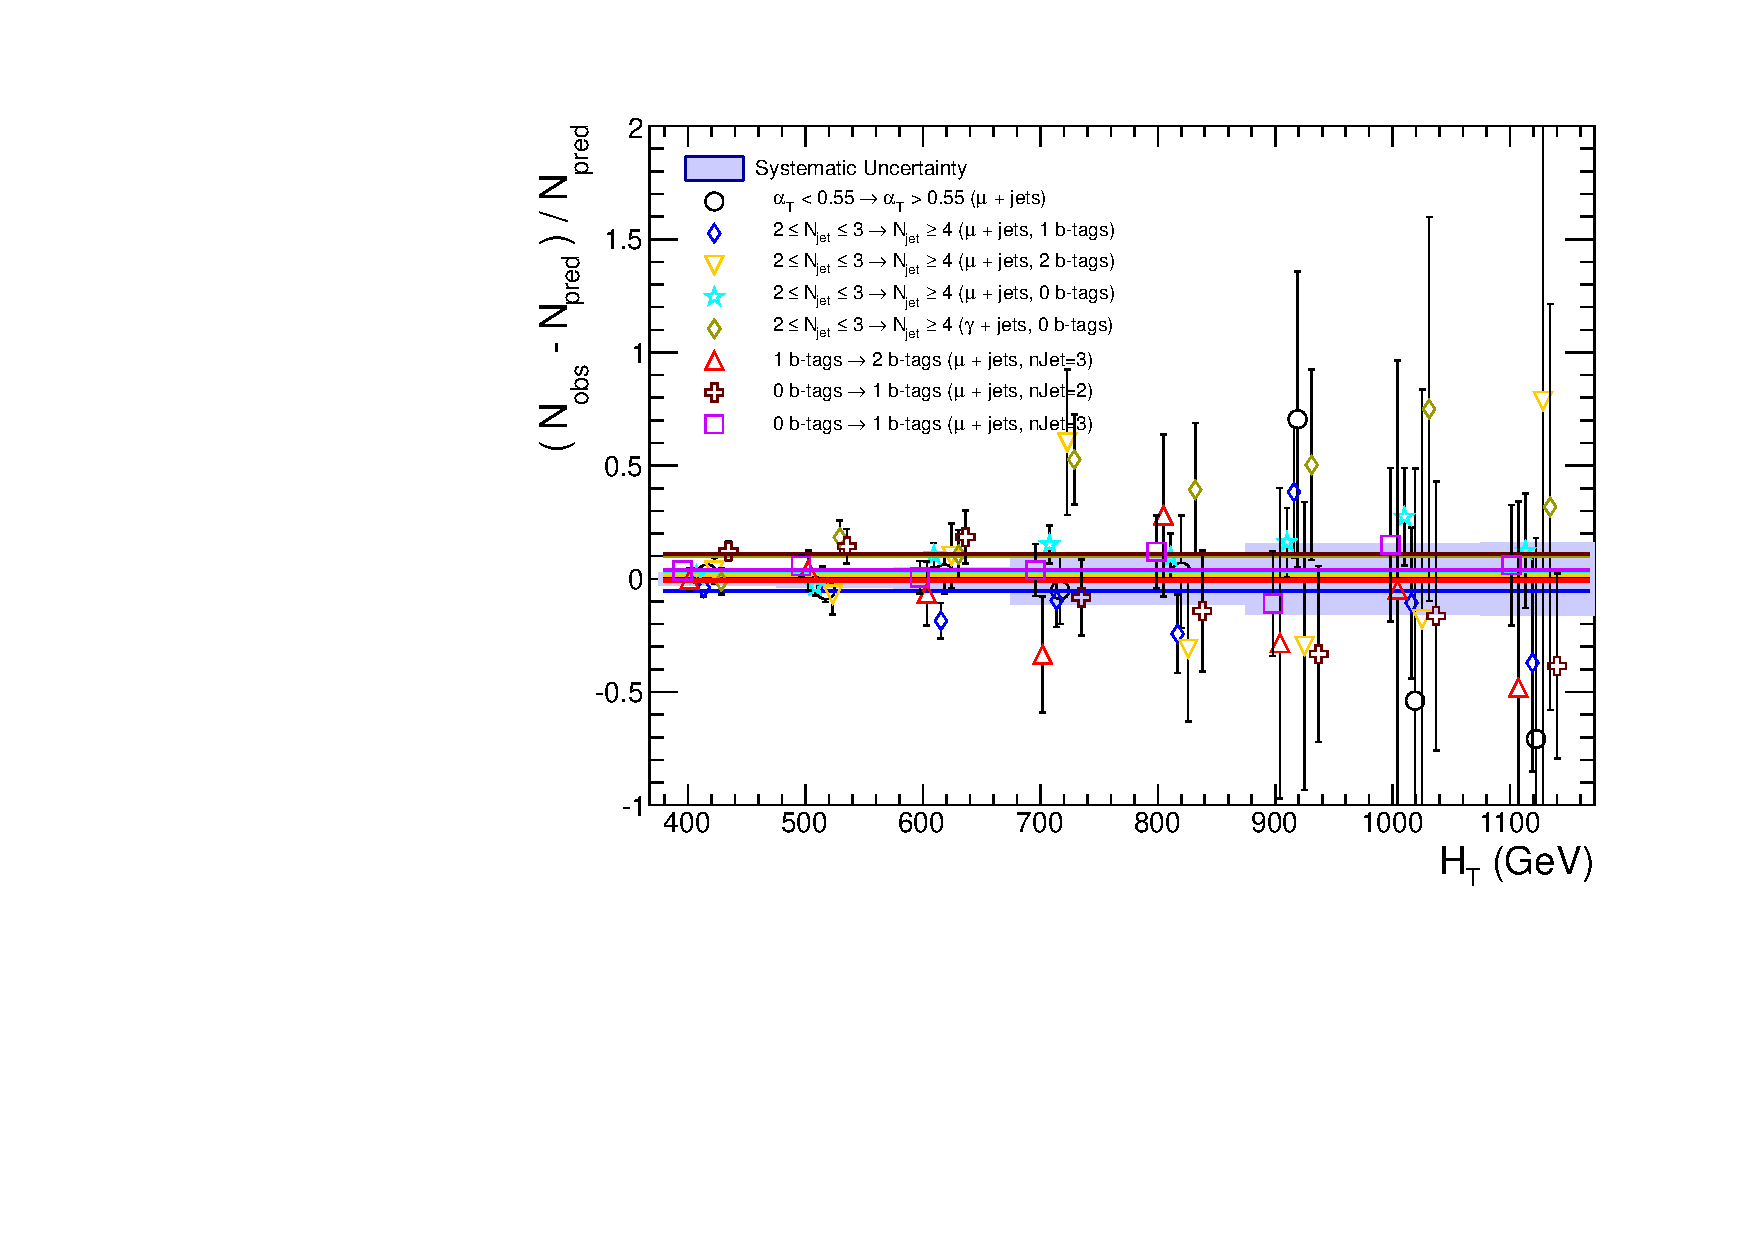
\includegraphics[width=0.7\textwidth]{figures/syst/closureTests_pf_take21_le3j.pdf}} \\
    \subfigure[$\njet \geq 4$]{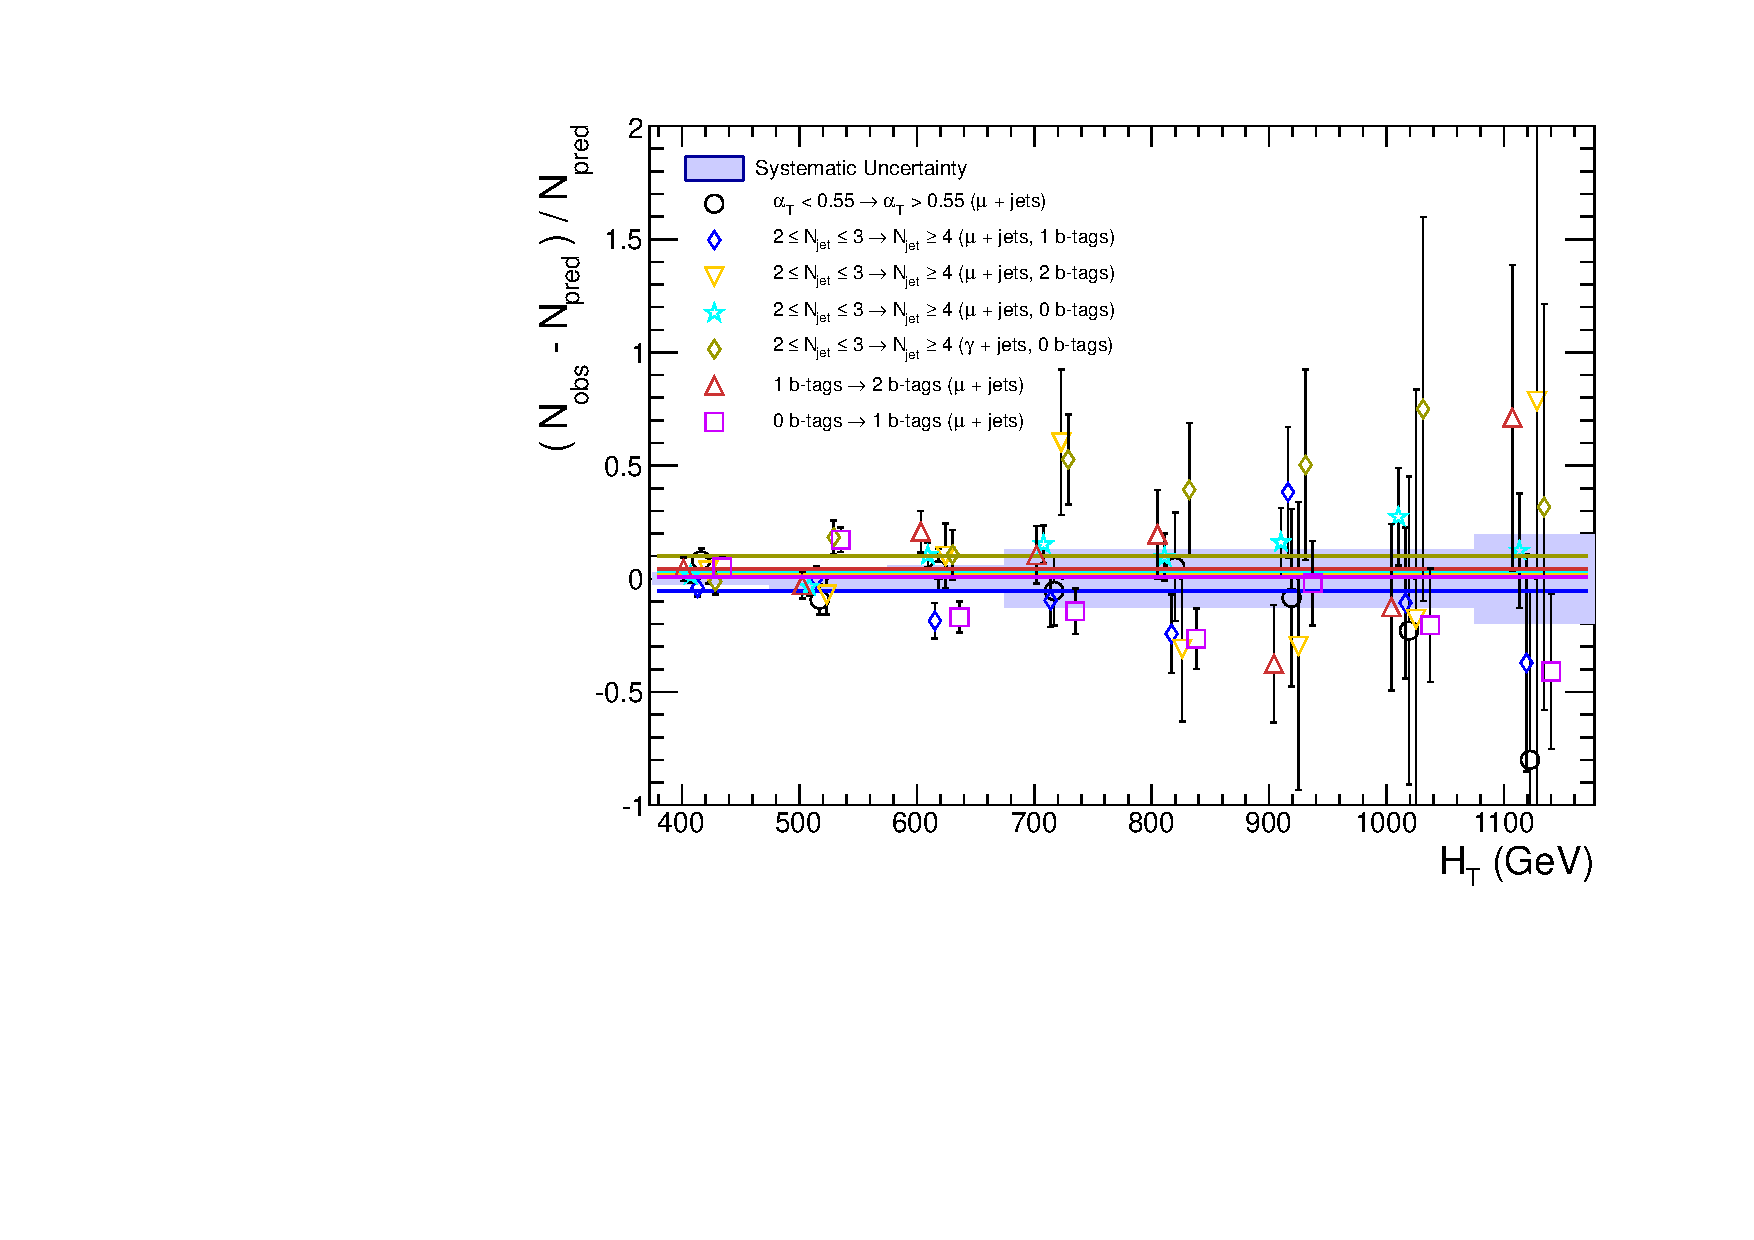
\includegraphics[width=0.7\textwidth]{figures/syst/closureTests_pf_take21_ge4j.pdf}} \\
    \caption{Sets of closure tests (open symbols) overlaid on top of
      the systematic uncertainty used for each of the \scalht
      region (shaded bands) and for the two different jet
      multiplicity bins: (a) $2 \leq \njet \leq 3$ and (b) $\njet \geq
      4$.  }
    \label{fig:closure}
  \end{center} 
\end{figure}

As described in Section~\ref{sec:muonSelection} the \alphat requirement is not imposed 
in the \mj control sample. Therefore it is important to verify the 
approach of using \mj samples without an \alphat requirement to 
make background predictions in the signal region.  The first set of
closure tests (denoted by circles) attempts to do this by probing
the modeling of the \alphat distribution in genuine \met events as a
function of \scalht.  The tests compares data yields in the \mj
sample with an \alphat requirement against predictions determined in a
\mj sample with the \alphat requirement inverted. 

The next three sets (triangles, crosses, squares) probe the
sensitivity of the transfer factors to the relative admixture of
events from the $W$ + jets and \ttbar processes. These tests are
conservative, since by construction, the admixture changes little when
translating from the \mj control region to the signal region, whereas the 
closure tests use sub-samples with different b-tag requirements and 
therefore have very different admixtures of W + jets and \ttbar events.  
In the \njetlow bin, the test is sub-divided into separate jet categories.
These tests also probe the modeling of the reconstruction of b-quark jets, 
although this also addressed more fully by dedicated studies that 
determine systematic uncertainties via the method described in
Section~\ref{sec:sms-syst-btag}.

The remaining tests probe the simulation modeling of
the jet multiplicity in the \mj and \gj samples, which is checked due 
to the exclusive binning in jet multiplicity. As in the case of the 
W + jets / \ttbar admixture, this set of tests  is a very conservative
 check, as predictions are always made from the same jet multiplicity bin,
whereas the closure tests translate between the two bins.

Tables~\ref{tab:syst-fits-le3j} and \ref{tab:syst-fits-ge4j}, which
summarize the results obtained from fits of zeroth order polynomials
(\ie a constant) to the sets of closure tests performed in the \njetlow 
and \njethigh bins.  Table~\ref{tab:syst-fits-njet} lists the fits result
common to both jet multiplicities. The best fit value and its uncertainty
is listed for each set of closure tests, along with the $\chi^{2}$, the number
of degrees of freedom, and the p-value of the fit. The best fit value
for the constant parameter is indicative of the level of closure, as
averaged across the full \scalht range considered in the analysis, and
the p-value is indicative of whether there is any significant
dependence on \scalht. 

The closure tests demonstrate, within the statistical precision 
of each test, that there are no significant biases or dependencies on 
\scalht inherent in the transfer factors obtained from simulation.  

One set of tests does indicate a poor goodness of fit (indicated by a
low p-value), which is the $\nb = 0 \ra \nb = 1$ test in the \mj
sample for the \njethigh category, which has been identified as a
upward (downward) fluctuation of event counts in the \scalht bin
475--575\gev (575--675\gev) when $\nb = 1$. Combining these two bins
yields an acceptable fit result, as indicated in
Table~\ref{tab:syst-fits-ge4j}, which points to a simple fluctuation
rather than any systematic bias.


\begin{table}[!h]
  \caption{A summary of the results obtained from fits of zeroth
    order polynomials (\ie a constant) to four sets of closure tests
    performed in the \njetlow bin.}
  \label{tab:syst-fits-le3j}
  \centering
  \footnotesize
  \begin{tabular}{ llrccc }
    \hline
    \hline
    &             & \multicolumn{4}{c}{Constant fit} \\
    \cline{3-6}
    Closure test  & Symbol & Best fit value & $\chi^2$ & d.o.f. & $p$-value \\
    \hline
    $\alphat < 0.55 \ra \alphat > 0.55$ (\mj) & Circle & $0.007 \pm 0.02$ & 3.91 & 7 & 0.79 \\ 
    1 b-tags \ra 2 b-tags (\mj, nJet=3) & Triangle & $-0.008 \pm 0.04$ & 3.20 & 7 & 0.87 \\ 
    0 b-tags \ra 1 b-tags (\mj, nJet=2) & Cross & $0.111 \pm 0.03$ & 5.87 & 7 & 0.55 \\ 
    0 b-tags \ra 1 b-tags (\mj, nJet=3) & Square & $0.040 \pm 0.02$ & 1.12 & 7 & 0.99 \\ 
    \hline
    \hline
  \end{tabular}
\end{table}

\begin{table}[!h]
  \caption{A summary of the results obtained from fits of zeroth
    order polynomials (\ie a constant) to three sets of closure tests
    performed in the \njethigh bin. $^{\dag} $Further explanation of this
    fit can be found in the text.}   
  \label{tab:syst-fits-ge4j}
  \centering
  \footnotesize
  \begin{tabular}{ llrccc }
    \hline
    \hline
    &             & \multicolumn{4}{c}{Constant fit} \\
    \cline{3-6}
    Closure test  & Symbol & Best fit value & $\chi^2$ & d.o.f. & $p$-value \\
    \hline
    $\alphat < 0.55 \ra \alphat > 0.55$ (\mj) & Circle & $0.011 \pm 0.04$ & 5.81 & 7 & 0.56 \\ 
    1 b-tags \ra 2 b-tags (\mj) & Triangle & $0.045 \pm 0.03$ & 9.36 & 7 & 0.23 \\ 
    0 b-tags \ra 1 b-tags (\mj) & Square & $0.007 \pm 0.03$ & 25.30 & 7 & 0.00 \\ 
    0 b-tags \ra 1 b-tags (\mj)$^{ \dag}$ & Square & $0.009 \pm 0.03$ & 10.12 & 6 & 0.12 \\ 
    \hline
    \hline
  \end{tabular}
\end{table}

\begin{table}[!h]
  \caption{A summary of the results obtained from fits of zeroth
    order polynomials (\ie a constant) to four sets of closure tests
    (\njetlow \ra \njethigh) that probe the accuracy of the MC
    modeling of the \njet distribution observed in data, using the
    three data control samples. } 
  \label{tab:syst-fits-njet}
  \centering
  \footnotesize
  \begin{tabular}{ llrccc }
    \hline
    \hline
    &             & \multicolumn{4}{c}{Constant fit} \\
    \cline{3-6}
    Closure test  & Symbol & Best fit value & $\chi^2$ & d.o.f. & $p$-value \\
    \hline
    \njetlow \ra \njethigh (\mj, 1 b-tags) & Times & $-0.053 \pm 0.03$ & 8.02 & 7 & 0.33 \\ 
    \njetlow \ra \njethigh (\mj, 1 b-tags) & Invert. Triangle & $0.018 \pm 0.04$ & 6.23 & 7 & 0.51 \\ 
    \njetlow \ra \njethigh (\mj, 0 b-tags) & Star & $0.034 \pm 0.02$ & 9.24 & 7 & 0.24 \\ 
    \njetlow \ra \njethigh (\gj, 0 b-tags) & Diamond & $0.100 \pm 0.04$ & 12.20 & 7 & 0.09 \\ 
    \hline
    \hline
  \end{tabular}
\end{table}


\subsection{Systematic uncertainties from closure tests\label{sec:syst-from-closure}}

Once it is established that no significantly large bias or trend is
observed for any set of closure tests, then systematic uncertainties
are determined. 

Systematics uncertainties are determined for each \scalht bin, as indicated in 
Table~\ref{tab:syst-values-from-ct}. For each \scalht region, the systematic
uncertainty is estimated by taking the quadrature sum of the weighted 
mean and sample variance for the closure tests within the given \scalht region.
This procedure yields the values quoted in Table~\ref{tab:syst-values-from-ct}.

As the closure tests do not translate from control region to signal region, they
do not probe the uncertainty in the signal trigger efficiencies.  To account for 
this, a trigger uncertainty of 5\% is added in quadrature to the uncertainty values obtained via the 
closure tests and the total is summarized in Table~\ref{tab:total-syst-values}.

\begin{table}[!h]
  \caption{A summary of the magnitude of the systematic uncertainties (\%) obtain
    from closure tests, according to \njet and \scalht region.}
  \label{tab:syst-values-from-ct}
  \centering
  \footnotesize
  \begin{tabular}{ ccccccccc }
    \hline
    \hline
            & \multicolumn{7}{c}{\scalht region (GeV)}                                \\
    \cline{2-9}
    \njet   & 375--475 & 475--525 & 525--675 & 675--775 & 775--875 & 875-975 & 1075-1075 & $>1175$ \\
    \hline                                                                                                                                  
    2--3    & 3        & 4        & 5        & 11       & 11       & 16      & 16        & 16     \\
    $\geq$4 & 3        & 4        & 6        & 13       & 13       & 13      & 13        & 20     \\
    \hline                                                                                                                                  
    \hline
  \end{tabular}
\end{table}


\begin{table}[!h]
  \caption{A summary of the magnitude of the total systematic uncertainties (\%)
    assigned to the transfer factors, according to \njet and \scalht
    region.}
  \label{tab:total-syst-values}
  \centering
  \footnotesize
  \begin{tabular}{ ccccccccc }
    \hline
    \hline
            & \multicolumn{7}{c}{\scalht region (GeV)}                                \\
    \cline{2-9}
    \njet   & 375--475 & 475--525 & 525--675 & 675--775 & 775--875 & 875-975 & 1075-1075 & $>1175$ \\
    \hline                                                                                                                                  
    2--3    & 6        & 6        & 7        & 12       & 12       & 17      & 17        & 17     \\
    $\geq$4 & 6        & 6        & 8        & 14       & 14       & 14      & 14        & 21     \\
    \hline                                                                                                                                  
    \hline
  \end{tabular}
\end{table}

Figure~\ref{fig:closure} shows the sets of closure tests overlaid on
top of gray bands that represent the \scalht-dependent systematic
uncertainties in Table~\ref{tab:syst-values-from-ct}. These systematic
uncertainties are assumed to fully uncorrelated between the different
b jet multiplicity categories and also the eight \scalht regions,
which is a conservative approach given that one can expect some
correlation between adjacent \scalht bins (due to comparable
kinematics).

